\documentclass[12 pt]{book}
\usepackage{amsmath, mathtools, amssymb}
\usepackage{amsthm}
\usepackage[paperwidth=5 in,paperheight=9 in,left=10 mm, right=10 mm, top=20 mm, bottom=20 mm]{geometry}
\usepackage{graphics}
\usepackage{fontawesome}
\usepackage{enumitem}
\usepackage{marvosym}
\newcommand{\myitem}{\refstepcounter{enumi}\item[$^\star$\theenumi.]}
\newcommand{\mmyitem}{\refstepcounter{enumi}\item[$^{\star \star}$\theenumi.]}
\setcounter{page}{1}
%\usepackage{watermark}


\usepackage[utf8]{inputenc}
\usepackage{xcolor}
\setlength{\arrayrulewidth}{0.1 mm}
%BLUE%
%\definecolor{Mycolor2}{HTML}{3D9BE9}
\definecolor{Mycolor2}{HTML}{33cccc}
%\definecolor{Mycolor2}{HTML}{000000}

%%----HEADER &&& FOOTER----%%

\usepackage{fancyhdr}

\pagestyle{fancy}
\fancyhf{}
\setlength{\headheight}{10 mm}
%\fancyhead[CE,CO]{\Large{\textbf{\textls*[385]{\textcolor{white}{ROTATION \\[-4 mm]{\normalsize{\textls*[500]{\textcolor{blackm}{EQUATION~\#\thepage}}}} \\[-12 mm]}}}}}


\renewcommand{\headrulewidth}{0 mm}
\renewcommand{\footrulewidth}{0 mm}


%%----FONT &&& MATHS_FONT----%%

\usepackage{amssymb}
\usepackage{upgreek,xspace}
\newcommand*{\rom}[1]{\expandafter\@\romannumeral #1}


\usepackage[utopia]{mathdesign}
\renewcommand{\familydefault}{\sfdefault}
\usepackage[scaled=1]{helvet}
\newcommand*\Times{\fontfamily{ptm}\selectfont}

%%%------PACAKAGES------%%%

\usepackage[letterspace=200]{microtype}
\usepackage{enumitem}
\usepackage{multicol}
\usepackage{pgfplots}
\pgfplotsset{width=8cm,compat=1.16}
\usepackage{tikz}
\usepgfplotslibrary{fillbetween}
\usetikzlibrary{quotes,angles,patterns,through,calc}
\usepgflibrary{arrows.meta}
\usetikzlibrary{optics}
\usetikzlibrary{intersections}

\usetikzlibrary{intersections}

\usepackage[version=4]{mhchem}
\usepackage{chemformula}
\usepackage{elements}

%\DeclareMathSymbol{\shortminus}{\mathbin}{AMSa}{"39}

\usepackage{mathtools}
\usepackage{old-arrows}
\usepackage[b]{esvect}

\newcommand{\midarrow}{\tikz \draw[-Stealth] (0,0) -- +(.1,0);}
\usetikzlibrary{mindmap}
\usetikzlibrary{scopes}
\usetikzlibrary{backgrounds}
\pgfsetlayers{background,main,foreground}
\pgfdeclarelayer{background}
\pgfdeclarelayer{foreground}
\usetikzlibrary{trees}
\usetikzlibrary{shadings}
%\tikzset{every node/.append style = {draw=black,thin}}
\usetikzlibrary{shadows}
\usetikzlibrary{chains}


\usepackage{color}
\usepackage[autostyle]{csquotes}


\usepackage{xcolor}
\definecolor{Mycolor2}{HTML}{33cccc}
\definecolor{One}{HTML}{336666}
\definecolor{Two}{HTML}{666666}
\definecolor{Three}{HTML}{cc6699}


%  black--brown--black %
\definecolor{Four}{HTML}{000000}
\definecolor{Five}{HTML}{330000}
\definecolor{Six}{HTML}{000000}

\definecolor{Seven}{HTML}{ff6666}
\definecolor{Eight}{HTML}{330066}
\definecolor{Nine}{HTML}{cc3333}
\definecolor{tomato}{HTML}{FF6347}
\definecolor{darkblue}{HTML}{2c3e50}
\definecolor{blackm}{HTML}{363636}
\definecolor{pink}{HTML}{ff6666}
\definecolor{c1}{HTML}{009999}
\definecolor{head}{HTML}{99ffff}
\definecolor{cyan}{HTML}{00eaff}




\newcommand{\sm}{\begin{minipage}[c]{0.1\linewidth}
{\Huge{\textcolor{tomato}{\textbf{ }}}}
\end{minipage}}



\newcommand\bonusspiral{} % just for safety
\def\bonusspiral[#1](#2)(#3:#4)(#5:#6)[#7]{% \bonusspiral[draw options](placement)(start angle:end angle)(start radius:final radius)[revolutions]
\pgfmathsetmacro{\domain}{#4+#7*360}
\pgfmathsetmacro{\growth}{180*(#6-#5)/(pi*(\domain-#3))}
\draw [#1,
       shift={(#2)},
       domain=#3*pi/180:\domain*pi/180,
       variable=\t,
       smooth,
       samples=int(\domain/5)] plot ({\t r}: {#5+\growth*\t-\growth*#3*pi/180})
}



\newcommand\irregularcircle[2]{% radius, irregularity
  \pgfextra {\pgfmathsetmacro\len{(#1)+rand*(#2)}}
  +(0:\len pt)
  \foreach \a in {10,20,...,350}{
    \pgfextra {\pgfmathsetmacro\len{(#1)+rand*(#2)}}
    -- +(\a:\len pt)
  } -- cycle
}



\newcommand{\AxisRotator}[1][rotate=0]{%
    \tikz [x=0.25cm,y=0.60cm,line width=.2ex,-stealth,#1] \draw (0,0) arc (-150:150:1 and 1);%
}



\def\centerarc[#1]#2(#3)#4(#5:#6:#7)% [draw options] (center) (initial angle:final angle:radius)
  {\draw[#1]($(#3)+({#7*cos(#5)},{#7*sin(#5)})$)arc(#5:#6:#7);}
 
 
 \tikzset{
kb1/.style={postaction={decorate,
   decoration={markings,mark=at position .5 with {\arrow{circled};}}}
   },
kb2/.style={postaction={decorate,
   decoration={markings,mark=at position .5 with {\arrow{Stealth};}}}
   },    
}
 

\tikzset{every to/.style={append after command={[draw,dashed]}}}

\tikzset{
  mirror->/.style={postaction={decorate,draw,thick,
decoration={border,amplitude=-0.25cm,angle=45,segment length=0.22cm}}
  }
}




\newcommand{\physics}{\normalsize{\textls*[100]{{\hspace*{75 mm} \textcolor{tomato}{\textsf{\textsc{@10xphysics}}}}}}}


\newenvironment{my-title}
{
	\begin{center}
	\begin{itshape}
	\large\Times\textit{}
}
{
	\end{itshape}
	\end{center}
}


\newenvironment{definition}
{
	\begin{center}
	\begin{itshape}
	\normalsize\Times\textit{}
}
{
	\end{itshape}
	\end{center}
}


\newenvironment{note}
{
	\begin{center}
	\begin{itshape}
	\normalsize\Times\textit{}
}
{
	\end{itshape}
	\end{center}
}



\begin{document}

\nopagecolor
%\fontseries{bx}
\boldmath
\setlength{\parindent}{0pt}
\color{white!100}
\Large


%%%%   EQUATION-01   %%%%%

\begin{my-title}
Moment Of Inertia
\end{my-title}

\begin{definition}
Moment of inertia gives a measurement of the resistance of a body to a change in its rotational motion.
\end{definition}

{\physics}

\begin{center}
\begin{tikzpicture}[xscale=1.5, yscale=1.25, ultra thick,line cap=round,every node/.style={scale=0.75}]
\draw (0,-2)--(0,2)node[below] {\AxisRotator[rotate=-90]};
\draw[dashed,very thick] (0,0)--(2,0) node[right]{$m$} node{${\small{\bullet}}$} node[midway, above]{$r$};
\end{tikzpicture}
\end{center}


\begin{note}
\tikz \node at (0,0)[scale=3]{$I = mr^2$};
\begin{align*}
m &- \textit{mass of the particle} \\
r &- \textit{distance from the axis} 
\end{align*}
\end{note}


\pagebreak




%%%%   EQUATION-02   %%%%%

\begin{my-title}
Moment of Inertia of a system of particles
\end{my-title}

{\physics}
 

\begin{center}
\begin{tikzpicture}[xscale=1.5, yscale=1.5, ultra thick,line cap=round,every node/.style={scale=0.75}]
\draw (0,-2)--(0,2)node[below] {\AxisRotator[rotate=-90]};
\draw[dashed,very thick] (0,1)--(2,1) node[right]{$m_1$} node{${\small{\bullet}}$} node[midway, above]{$r_1$};
\draw[dashed,very thick] (0,0)--(2.5,0) node[right]{$m_2$} node{${\small{\bullet}}$} node[midway, above]{$r_2$};
\draw[dashed,very thick] (0,-1)--(-2,-1) node[left]{$m_3$} node{${\small{\bullet}}$} node[midway, above]{$r_3$};
\end{tikzpicture}
\end{center}


\begin{note}
\tikz \node at (0,0)[scale=3]{$I =\Sigma m_i r^2_i$};
\begin{align*}
m &- \textit{mass of the particle} \\
r &- \textit{distance from the axis} 
\end{align*}
\end{note}

\pagebreak





%%%%   EQUATION-03   %%%%%


\begin{my-title}
Moment of Inertia of rigid bodies
\end{my-title}

\Times \large\textit{\textcolor{black}{Moment if inertia gives a measurement of the resistance of a body to a change in its rotational motion.}}

{\physics}

\begin{note}
\tikz \node at (0,0)[scale=3.3]{$I =\int r^2 \; dm$};
\begin{align*}
dm &- \textit{differential mass} \\
r &- \textit{position of $dm$} 
\end{align*}
\end{note}


\pagebreak



%%%%   EQUATION-04   %%%%%

\begin{my-title}
Moment of Inertia of ring
\end{my-title}

\begin{definition}
Moment of inertia of a ring about an axis passing through its centre and perpendicular to the plane of the ring.
\end{definition}

{\physics}

\begin{center}
\begin{tikzpicture}[xscale=1.25, yscale=1, ultra thick,line cap=round,every node/.style={scale=0.75}]
\draw (0,-2)--(0,2)node[below] {\AxisRotator[rotate=-90]};
\draw (0,0) ellipse[x radius=1.75, y radius=0.55];
\draw[dashed,very thick] (0,0)--(1.75,0) node[right]{$m$} node{${\small{\bullet}}$} node[midway, above]{$r$};
\end{tikzpicture}
\end{center}


\[
I = mr^2
\]

\begin{note}
$m$ - mass of the ring, \quad \quad $r$ - radius of the ring
\end{note}

\pagebreak



%%%%   EQUATION-05  %%%%%

\begin{my-title}
Moment of Inertia of hollow cylinder
\end{my-title}

\begin{definition}
Moment of inertia of a hollow cylinder about its axis.
\end{definition}

{\physics}

\begin{center}
\begin{tikzpicture}[xscale=1.2, yscale=1.2, ultra thick,line cap=round,every node/.style={scale=0.75}]
\draw[dashed,thick] (0,-2)--(0,2) node[below] {\AxisRotator[rotate=-90]};
\draw[very thick] (0,0.75) ellipse[x radius=1, y radius=0.45];
\draw[very thick] (0,-0.75) ellipse[x radius=1, y radius=0.45];
\draw[very thick] (1,0.75)--(1,-0.75);
\draw[very thick] (-1,0.75)--(-1,-0.75);
\draw[-Stealth,thick] (0,0.75)--(1,0.75)  node[midway, above]{$r$};
\end{tikzpicture}
\end{center}

\[
I = mr^2
\]

\begin{note}
$m$ - mass of the cylinder, \quad \quad $r$ - radius of the cylinder
\end{note}

\pagebreak




%%%%   EQUATION-06  %%%%%

\begin{my-title}
Moment of Inertia of disc
\end{my-title}

\begin{definition}
Moment of inertia of a disc about an axis passing through its centre and perpendicular to the plane of the disc.
\end{definition}

{\physics}

\begin{center}
\begin{tikzpicture}[xscale=1.1, yscale=0.95, ultra thick,line cap=round,every node/.style={scale=0.75}]
\draw (0,-2)--(0,2)node[below] {\AxisRotator[rotate=-90]};
\draw [thick,fill=black!65,opacity=0.75](0,0) ellipse[x radius=1.75, y radius=0.55];
\draw[-Stealth,thick] (0,0)--(1.75,0) node[midway, above]{$r$};
\end{tikzpicture}
\end{center}

\[
I = \dfrac{mr^2}{2}
\]

\begin{note}
$m$ - mass of the disc, \quad \quad $r$ - radius of the disc
\end{note}

\pagebreak



%%%%   EQUATION-07  %%%%%

\begin{my-title}
Moment of Inertia of sphere
\end{my-title}

\begin{definition}
Moment of inertia of a solid sphere about an axis passing through it's centre.
\end{definition}

{\physics}

\begin{center}
\begin{tikzpicture}[rotate=15,scale=0.75,thick,line cap=round,every node/.style={scale=0.5}]
  \draw[very thick] (0,-2.7)--(0,2.8)node[below] {\AxisRotator[rotate=-75]};
  \shade[ball color = gray!40, opacity = 0.4] (0,0) circle (2cm);
  \draw (0,0) circle (2cm);
  \draw (-2,0) arc (180:360:2 and 0.6);
  \draw[dashed] (2,0) arc (0:180:2 and 0.6);
  \fill[fill=black] (0,0) circle (1pt);
  \draw[dashed] (0,0 ) -- node[above]{$r$} (2,0);
\end{tikzpicture}
\end{center}

\[
I = \dfrac{2}{5} \, mr^2
\]

\begin{note}
$m$ - mass of the sphere, \quad \quad $r$ - radius
\end{note}


\pagebreak



\begin{my-title}
Moment of Inertia of a uniform rod
\end{my-title}


\begin{definition}
About an axis passing through one of it's end.
\end{definition}

\begin{center}
\begin{tikzpicture}[scale=0.9,very thick, >=Stealth,every node/.style={scale=0.7}]
\draw[thick] (0,-1.7)--(0,2)node[below] {\AxisRotator[rotate=-90]};
\draw[dashed,->,thick]  (0,0)--(5.5,0)node[right]{$x$};
\draw[thick] (0,0) -- (4,0) --  (4,0.25) -- (0,0.25) -- cycle;
\fill[even odd rule, fill=white] (2.23,0) -- (2.62,0)--(2.62,0.25) -- (2.23,0.25) -- cycle;
\draw[thick,->] (0,-0.45)--(2.1,-0.45) node[right=-1.5 mm]{$dx$} node[midway, below]{$x$};
\draw[thick] (0,0.25) to[dim arrow={label=$l$}] (4,0.25);
\end{tikzpicture}
\end{center}

{\physics}

\begin{boldmath}
\[
I = \dfrac{ml^2}{3} 
\]
\end{boldmath}

\begin{note}
$m$ - mass of the rod, \quad \quad $l$ - length of the rod
\end{note}

\pagebreak


\begin{my-title}
Moment of Inertia of a solid cone
\end{my-title}

\begin{definition}
Moment of Inertia of a solid cone about an axis passing\\[-2 mm] through its centre of mass and perpendicular to the base.
\end{definition}

\vspace{-5 mm}

{\physics}

\begin{center}
\begin{tikzpicture}[yscale=0.75,very thick, >=Stealth,every node/.style={scale=0.7}]
\draw[dashed,thick] (0,0) arc (170:10:2cm and 0.4cm)coordinate[pos=0] (a);
    \draw (0,0) arc (-170:-10:2cm and 0.4cm)coordinate (b);
    \draw[densely dashed,thick] ([yshift=4cm]$(a)!0.5!(b)$) -- node[right] {$h$}coordinate[pos=0.95] (aa)($(a)!0.5!(b)$)
                            -- node[above] {$r$}coordinate[pos=0.1] (bb) (b);
    \draw (aa) -| (bb);
    \draw (a) -- ([yshift=4cm]$(a)!0.5!(b)$) -- (b);
    \draw[thick] (2,-1.1)--(2,4.75)node[below] {\AxisRotator[rotate=-90]};
\end{tikzpicture}
\end{center}

\begin{boldmath}
\[
I = \dfrac{3}{10} mr^2
\]
\end{boldmath}

\begin{note}
$m$ - mass of the cone, \quad \quad $r$ - radius
\end{note}

\pagebreak


\begin{my-title}
parallel axes theorem for moment of inertia
\end{my-title}

{\physics}

\begin{center}
\begin{tikzpicture}[scale=1.25,very thick,every node/.style={scale=0.7}]
  \coordinate (c) at (0,0);
  \coordinate (d) at (1,2);
  \draw[ultra thick, rounded corners=1mm] (d) \irregularcircle{1cm}{1mm};
 \draw[thick] (1,0.25)--(1,4)node[below] {\AxisRotator[rotate=-90]};
  \draw[thick] (3,0.25)--(3,4)node[below] {\AxisRotator[rotate=-90]};
  \node at (1,2) {$\bullet$};
  \node at (1,2)[left] {COM};
  \draw[thick] (1,0.2) to [dim arrow={label=$r$}] (3,0.2);
\end{tikzpicture}
\end{center}

\begin{boldmath}
\[
I = I_{\textit{COM}}  \; + \;  mr^2
\]
\end{boldmath}

\begin{note}
$I$ - moment of inertia about the new axis  \\ $m$ - mass , \quad \quad $r$ - distance between the parallel axes
\end{note}

\pagebreak


\begin{my-title}
perpendicular axes theorem for moment of inertia
\end{my-title}

\begin{center}
\begin{tikzpicture}[scale=1.25, thick,every node/.style={scale=0.7}]
\draw[ultra thick, rounded corners=1mm] (0.25,0.25) \irregularcircle{1cm}{1mm};
\draw[-Stealth] (0,0,0)--(3,0,0) node[below]{$X$};
\draw[-Stealth] (0,0,0)--(0,2.25,0) node[left]{$Z$};
\draw[-Stealth] (0,0,0)--(1,0,-2) node[above]{$Y$};
%\draw (0.5,0,0) arc[start angle=0, end angle=24, radius=0.5];
%\draw [line width=0 mm, opacity=0.35,pattern=grid, pattern color=white!35] (0,0,0)--(2,0,0)--(3,0,-2)--(1,0,-2)--(0,0,0);
\end{tikzpicture}
\end{center}

{\physics}

\begin{boldmath}
\[
I_Z = I_X  \; + \;  I_Y
\]
\end{boldmath}

\vspace*{-5 mm}

\begin{note}
This theorem is applicable only to the plane bodies (2D).\\
$X$ and $Y$ axes chosen in the plane of the body and $Z$-axis perpendicular to this plane, three axes being mutually perpendicular.
\end{note}

\pagebreak



\begin{my-title}
moment of inertia of rectangular slab
\end{my-title}

\begin{center}
\begin{tikzpicture}[scale=1.15, thick,every node/.style={scale=0.7}]
\draw[thick](0,-2)-- (0, 0);
\draw[thick, pattern=grid, pattern color=black!35] (-3,-1) coordinate(a) -- (2 , -1) coordinate(b) -- (3,1) coordinate(c) -- (-2, 1) coordinate(d)--cycle;
\begin{scope}[xshift=1,yshift=-2]
\draw[thick, pattern=grid, pattern color=black!35] (-3,-1) coordinate(a) -- (2 , -1) coordinate(b) -- (3,1) coordinate(c) -- (-2, 1) coordinate(d)--cycle;
\end{scope}
\draw (c) to [dim arrow={label=$b$}] (b);
\draw (a)++(0,-1) to [dim arrow={label'=$a$}] ($(b)+(0,-1)$);
\draw[thick](0, 0) node{$\bullet$}--(0, 2.25) node[below] {\AxisRotator[rotate=-90]};
\end{tikzpicture}
\end{center}

{\physics}

\begin{boldmath}
\[
I = \dfrac{m}{12} \left( a^2 + b^2 \right)
\]
\end{boldmath}




\pagebreak




\begin{my-title}
angular momentum
\end{my-title}

\begin{center}
\begin{tikzpicture}[>=Stealth,scale=1,very thick,every node/.style={scale=0.8},decoration={
    markings,
    mark=at position 0.59 with {\arrow{Stealth}}}]
\centerarc [very thick] (0,0)(10:100:3);
\draw[->,postaction={decorate}](0,0) node{$\bullet$}-- ([turn]140:3) node[midway, below]{$\vec{r}$} node{$\bullet$} -- ([turn]90:2) node[midway,right=3 mm,above]{$\vec{p}$};
\end{tikzpicture}
\end{center}

{\physics}

\begin{boldmath}
\[
\vec{L} = \vec{r} \times \vec{p}
\]
\end{boldmath}

\begin{note}
$\vec{r}$ - position vector \quad \quad $\vec{p}$ - linear momentum
\end{note}

\pagebreak

\begin{my-title}
angular momentum
\end{my-title}

{\physics}

\begin{align*}
\vec{L} &= \vec{r} \times \vec{p} \\[2 mm]
			&= \vec{r} \times m \left( \vec{\omega} \times \vec{r} \right) \\[2 mm]
			&= m \left[ \vec{r} \times \left( \vec{\omega} \times \vec{r} \right) \right] \\[2 mm]
			&= m \left[ \left( \vec{r} \cdot \vec{r} \right) \vec{\omega}  -  \left( \vec{r} \cdot \vec{\omega} \right) \vec{r} \right] \\[2 mm]
			&= m \left[ r^2 \vec{\omega}  -  0 \right] \\[2 mm]
			&= mr^2 \vec{\omega} \\[2 mm]
\vec{L} &= I \vec{\omega}
\end{align*}

\pagebreak


\begin{my-title}
work done due to torque
\end{my-title}

\begin{align*}
dW &=  \vec{F} \cdot d\vec{l} \\[4 mm]
	   &=  \vec{F} \cdot \left( d\vec{\theta} \times \vec{r} \right) \\[4 mm]
	   &=  \left( \vec{r} \times \vec{F} \right) \cdot d\vec{\theta} \quad {\small{\textit{scalar triple product}}} \\[4 mm]
dW &=  \vec{\tau} \cdot d\vec{\theta} \\[4 mm]
W	  &= \int_{\theta_i}^{\theta_f} \vec{\tau} \cdot d\vec{\theta} \\
\end{align*}

{\physics}


\pagebreak


\begin{my-title}
angular impulse
\end{my-title}

\begin{align*}
\upphi &= \int_{t_i}^{t_f} \tau \; dt \\[2 mm]
		   &= \int I\upalpha \; dt \\[2 mm]
		   &= \int I \; \dfrac{d\omega}{dt} \; dt \\[2 mm]
		   &= \int_{\omega_i}^{\omega_f} I \; d\omega \\[2 mm]
\upphi_{\textit{net}} &= \Delta L
\end{align*}

{\physics}

\pagebreak


\begin{my-title}
acceleration on inclined plane
\end{my-title}

\begin{center}
\begin{tikzpicture}[very thick, scale=1,>=Stealth,every node/.style={scale=0.8}]
\draw [mirror->] (0,0)--(5,0) coordinate (d) (1,0) coordinate (a) --([turn]45:5) coordinate (b);
\coordinate (c) at ($(a)!0.7!(b)$);
\draw (c) - - ($(c)!1cm!90:(b)$) coordinate (o) edge[->] node[at end,left]{$mg\sin\theta$} ([turn]90:2) circle(1cm);
\centerarc [->, thick] (o)(-60:190:0.4);
\fill (o) circle(1.8pt);
\pic [draw=white,"$\theta$", angle eccentricity=1.6,angle radius=0.8 cm] {angle = d--a--b};
\end{tikzpicture}
\end{center}

{\physics}

\begin{boldmath}
\[
a = \dfrac{g\sin\theta}{1 + \dfrac{I_{\textit{CM}}}{mr^2}}
\]
\end{boldmath}

\begin{note}
$I_{\textit{CM}}$ - moment of inertia about centre of mass  \quad \quad $r$ - radius
\end{note}

\pagebreak



\begin{my-title}
minimum coefficient of friction required for pure rolling motion on inclined plane
\end{my-title}

\begin{center}
\begin{tikzpicture}[very thick, scale=1,>=Stealth,every node/.style={scale=0.8}]
\draw [mirror->] (0,0)--(5,0) coordinate (d) (1,0) coordinate (a) --([turn]45:5) coordinate (b);
\coordinate (c) at ($(a)!0.7!(b)$);
\draw (c) - - ($(c)!1cm!90:(b)$) coordinate (o) edge[->] node[at end,left]{$mg\sin\theta$} ([turn]90:2) circle(1cm);
\centerarc [->, thick] (o)(-60:190:0.4);
\fill (o) circle(1.8pt);
\pic [draw=white,"$\theta$", angle eccentricity=1.6,angle radius=0.8 cm] {angle = d--a--b};
\end{tikzpicture}
\end{center}

{\physics}

\begin{boldmath}
\[
\upmu \geq \dfrac{\tan\theta}{1 + \dfrac{mr^2}{I_{\textit{CM}}}}
\]
\end{boldmath}

\pagebreak

\begin{my-title}
friction force
\end{my-title}

\begin{center}
\begin{tikzpicture}[very thick, scale=1,>=Stealth,every node/.style={scale=0.8}]
\draw [mirror->] (0,0)--(5,0) coordinate (d) (1,0) coordinate (a) --([turn]45:5) coordinate (b);
\coordinate (c) at ($(a)!0.7!(b)$);
\draw (c) - - ($(c)!1cm!90:(b)$) coordinate (o) edge[->] node[at end,left]{$mg\sin\theta$} ([turn]90:2) circle(1cm);
\centerarc [->, thick] (o)(-60:190:0.4);
\fill (o) circle(1.8pt);
\pic [draw=white,"$\theta$", angle eccentricity=1.6,angle radius=0.8 cm] {angle = d--a--b};
\draw [->,red] (c)--++(1.75,1.75) node[above]{$f_r$};
\end{tikzpicture}
\end{center}

{\physics}

\begin{boldmath}
\[
f_r = \dfrac{mg\sin\theta}{1 + \dfrac{mr^2}{I_{\textit{CM}}}}
\]
\end{boldmath}

\pagebreak

\end{document}